\section{Experience}
\label{sect:results}

The \blockchain\ went live on November 28th, 2018. For the curious reader, there is a timestamp in each block and the first mined key-block has timestamp ``1543373685748'', which is the time in milliseconds using POSIX time. Since that first date, 3 major protocol updates have successfully be applied, enriching the \blockchain\ with new features. The new protocols are effective at a certain height and the software supports the old protocol under that height and the new protocol from that height. Each protocol is refered to by name for ease in communication with developers of blockchain applications: \textit{Roma}, effective at height 0, \textit{Minerva}, effective at height 47800, \textit{Fortuna}, effective at height 90800, and \textit{Lima}, effective at height 161150.

The blockchain has slowly attracted more traffic and we can now see over 1000 transactions an hour on busy days (Fig.\ \ref{txs-nrs}).
\begin{figure}[h]
   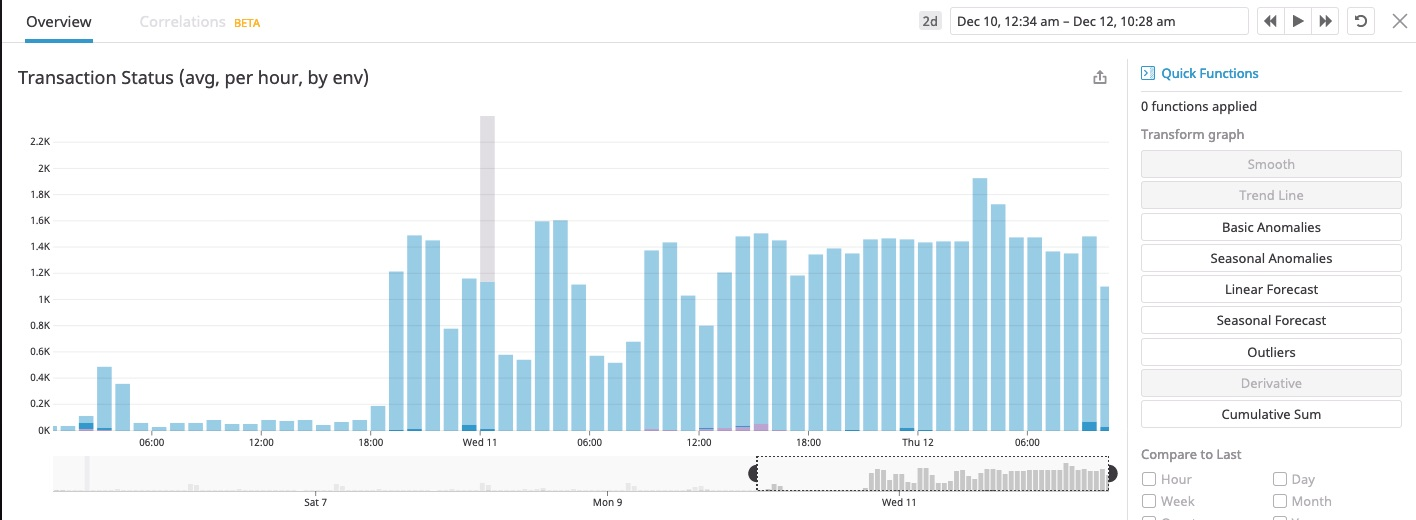
\includegraphics[scale=0.23]{TransactionsDec2019.jpg}
   \caption{Transaction status}
   \label{txs-nrs}
\end{figure}
This is much below the theoretical maximum of 100 on-chain transaction per second.

The confirmation time of transactions is the time between posting the transaction and seeing it in a micro-block on chain. We measure this over a longer time by posting a transaction each 3 seconds carrying the post time as timestamp in the payload. The micro-block in which this transaction appears also has a timestamp (set by the clock of the miner). The difference is observable for everyone, since these are transactions on chain. The mean of confirmation times is around the expected 3 seconds.

At height 183490 we had the following totals of different transaction types:

\begin{center}
\begin{tabular}{l|lcl|l}
        Transaction Type     &  count  & \vspace{2mm} & Transaction Type     &  count  \\
  \hline
  SpendTx      &  4117919  &  & ChannelCloseMutualTx   &      15  \\
 GAAttachTx             &       2  &  & ChannelCloseSoloTx     &      3  \\
 GAMetaTx               &       5  &  & ChannelCreateTx        &    119  \\
 NameClaimTx            &  557012  & & ChannelDepositTx       &       2  \\
 NamePreclaimTx         &  605026  & & ChannelForceProgressTx &       1  \\
 NameRevokeTx           &      1  & & ChannelSettleTx        &       2  \\
  NameTransferTx         &      59  & & ChannelSlashTx         &       1  \\
  NameUpdateTx           & 431037  & & ChannelSnapshotSoloTx  &       1  \\
  OracleExtendTx        &     276  & &  ChannelWithdrawTx      &       1  \\
  OracleQueryTx          &     603  & &  ContractCallTx         &   48063  \\
  OracleRegisterTx       &      25  && ContractCreateTx       &     259  \\
 OracleResponseTx       &     590  \\
\end{tabular}
\end{center}

 Which clearly shows that oracles are less popular than the naming system\footnote{Since the Lima release, name auctions are introduced, invalidating the names in the \texttt{.test} domain. Most name transactions are from before this release.}. It also shows that the state channels have not yet started to be widely used, but there are clearly some contracts that are heavily called.
